% Generated from the public primitive catalog. Original Atlas drawing; Apache-2.0.
% Target: aes-128; view: detail
\documentclass[border=9pt]{standalone}
% Original Atlas figure theme. Apache-2.0; see the repository LICENSE.
\usepackage[T1]{fontenc}
\usepackage{lmodern}
\usepackage{amsmath,amssymb}
\usepackage{tikz}
\usetikzlibrary{arrows.meta,positioning,calc,fit,backgrounds,decorations.pathreplacing,matrix}
\definecolor{atlasInk}{HTML}{172235}
\definecolor{atlasTeal}{HTML}{0D7B7D}
\definecolor{atlasMuted}{HTML}{637278}
\definecolor{atlasFill}{HTML}{EAF4F2}
\definecolor{atlasLine}{HTML}{B6C8C7}
\tikzset{
  every picture/.style={line width=.65pt,draw=atlasInk,>=Latex},
  every node/.style={text=atlasInk,font=\sffamily\small},
  box/.style={draw,rounded corners=1.5pt,minimum height=.9cm,minimum width=1.6cm,align=center,inner sep=6pt,fill=white},
  accent/.style={box,draw=atlasTeal,fill=atlasFill},
  wire/.style={->,line width=.7pt},
  keywire/.style={wire,draw=atlasTeal,dashed},
  xor/.style={draw,circle,fill=white,inner sep=0pt,minimum size=.38cm},
  add/.style={draw,rectangle,fill=white,inner sep=0pt,minimum size=.38cm},
  note/.style={font=\sffamily\scriptsize,text=atlasMuted,align=center},
  phase/.style={font=\sffamily\small\bfseries,text=atlasTeal},
  group/.style={draw=atlasLine,dashed,rounded corners=2pt,inner sep=8pt}
}
\newcommand{\rotl}{\mathbin{\lll}}
\newcommand{\rotr}{\mathbin{\ggg}}
\newcommand{\kx}{\operatorname{Keccak}\!\text{-}\!f[1600]}

\newcommand{\AtlasKeyBits}{128}
\newcommand{\AtlasKeyWords}{4}
\newcommand{\AtlasRounds}{10}
\newcommand{\AtlasPriorRounds}{9}
\newcommand{\AtlasRoundKeys}{11}
\newcommand{\AtlasDoubleRounds}{5}
\newcommand{\AtlasSixRoundGroups}{1.6666666666666667}
\newcommand{\AtlasFLGroups}{0.6666666666666667}
\newcommand{\AtlasRoundStart}{14}
\newcommand{\AtlasBlockBits}{128}
\newcommand{\AtlasOutputBits}{d}
\newcommand{\AtlasStateBits}{8w}
\newcommand{\AtlasNonceBits}{v}
\newcommand{\AtlasCounterBits}{q}
\newcommand{\AtlasStreamBlockBits}{b}
\newcommand{\AtlasRate}{r}
\newcommand{\AtlasCapacity}{c}
\newcommand{\AtlasSteps}{N}
\newcommand{\AtlasLastStep}{N-1}
\newcommand{\AtlasWordBits}{w}
\newcommand{\AtlasHashWords}{h}
\newcommand{\AtlasFeedForward}{\boxplus}
\newcommand{\AtlasByteOrder}{big-endian}
\newcommand{\AtlasDomain}{01}
\newif\ifAtlasXof
\AtlasXoffalse
\begin{document}
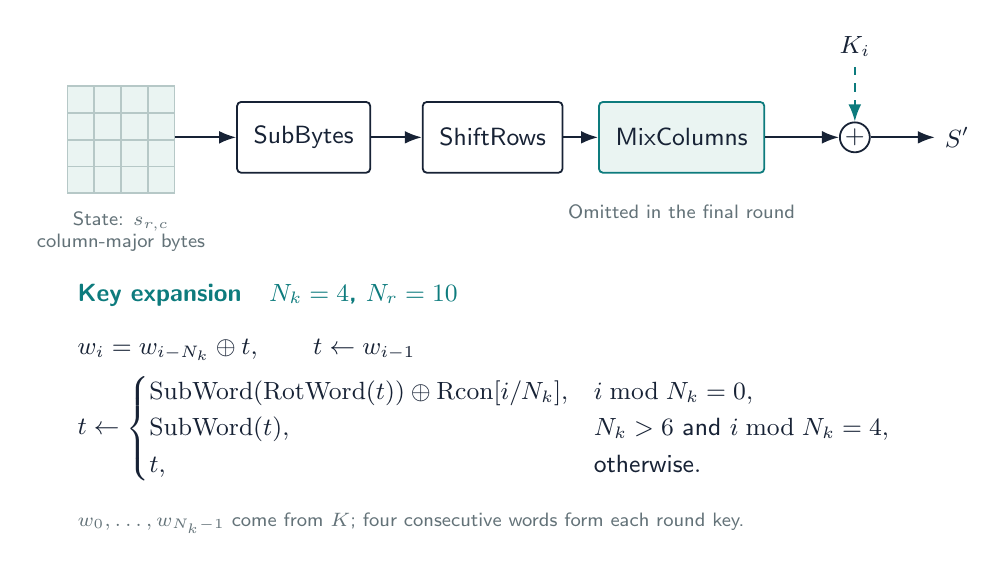
\begin{tikzpicture}
  \foreach \x in {0,...,3} \foreach \y in {0,...,3} {
    \draw[draw=atlasLine,fill=atlasFill] (.34*\x,1.5-.34*\y) rectangle ++(.34,-.34);
  }
  \node[note] at (.68,-.35) {State: $s_{r,c}$\\column-major bytes};
  \node[box] (sb) at (3, .85) {SubBytes};
  \node[box] (sr) at (5.4, .85) {ShiftRows};
  \node[accent] (mc) at (7.8, .85) {MixColumns};
  \node[xor] (ak) at (10, .85) {$+$};
  \node (out) at (11.3, .85) {$S'$};
  \draw[wire] (1.36,.85) -- (sb);
  \draw[wire] (sb) -- (sr); \draw[wire] (sr) -- (mc);
  \draw[wire] (mc) -- (ak); \draw[wire] (ak) -- (out);
  \node (rk) at (10,2) {$K_i$}; \draw[keywire] (rk) -- (ak);
  \node[note] at (7.8,-.1) {Omitted in the final round};
  \node[phase,anchor=west] at (0,-1.15) {Key expansion\quad $N_k=\AtlasKeyWords$, $N_r=\AtlasRounds$};
  \node[anchor=west] at (0,-1.85) {$w_i=w_{i-N_k}\oplus t,\qquad t\gets w_{i-1}$};
  \node[anchor=west] at (0,-2.85) {$t\gets\begin{cases}
    \operatorname{SubWord}(\operatorname{RotWord}(t))\oplus\operatorname{Rcon}[i/N_k],&i\bmod N_k=0,\\
    \operatorname{SubWord}(t),&N_k>6\ \text{and}\ i\bmod N_k=4,\\
    t,&\text{otherwise}.
  \end{cases}$};
  \node[note,anchor=west] at (0,-4.05) {$w_0,\ldots,w_{N_k-1}$ come from $K$; four consecutive words form each round key.};
\end{tikzpicture}

\end{document}
